\documentclass[10pt,twocolumn,letterpaper]{article}

\usepackage{cvpr}
\usepackage{times}
\usepackage{epsfig}
\usepackage{graphicx}
\usepackage{amsmath}
\usepackage{amssymb}
\usepackage{enumitem}

% Include other packages here, before hyperref.

% If you comment hyperref and then uncomment it, you should delete
% egpaper.aux before re-running latex.  (Or just hit 'q' on the first latex
% run, let it finish, and you should be clear).
\usepackage[breaklinks=true,bookmarks=false]{hyperref}

\cvprfinalcopy % *** Uncomment this line for the final submission

\def\cvprPaperID{****} % *** Enter the CVPR Paper ID here
\def\httilde{\mbox{\tt\raisebox{-.5ex}{\symbol{126}}}}

% Pages are numbered in submission mode, and unnumbered in camera-ready
%\ifcvprfinal\pagestyle{empty}\fi
\setcounter{page}{1}
\begin{document}

%%%%%%%%% TITLE
\title{Deep Dish : Deep Learning on a Platter}

\author{Abhishek Goswami\\
Microsoft\\
Redmond, WA\\
{\tt\small agoswami@microsoft.com}
% For a paper whose authors are all at the same institution,
% omit the following lines up until the closing ``}''.
% Additional authors and addresses can be added with ``\and'',
% just like the second author.
% To save space, use either the email address or home page, not both
\and
Haichen Liu\\
{\tt\small haichen.sjtu@gmail.com}
}

\maketitle
%\thispagestyle{empty}

%%%%%%%%% ABSTRACT
\begin{abstract}
   %The ABSTRACT is to be in fully-justified italicized text, at the top
   %of the left-hand column, below the author and affiliation
   %information. Use the word ``Abstract'' as the title, in 12-point
   %Times, boldface type, centered relative to the column, initially
   %capitalized. The abstract is to be in 10-point, single-spaced type.
   %Leave two blank lines after the Abstract, then begin the main text.
   %Look at previous CVPR abstracts to get a feel for style and length.
	
	We consider applying deep convolutional neural networks on images of food dishes. Food items have unique characteristics - they come in different colors and shapes, can be clustered into groups (e.g. fruits, vegetables), and food items can be combined in several ways to prepare a meal etc. This makes images of food dishes particularly suitable for visual recognition tasks.
		
\end{abstract}

%%%%%%%%% BODY TEXT
\section{Introduction}

%Explain the problem and why it is important. Discuss your motivation for pursuing this problem. Give some background if necessary. Clearly state what the input and output is. Be very explicit: "The input to our algorithm is a {satellite image, YouTube video, patient age, 3D video, etc.}. We then use a {CNN, LSTM, GAN, etc.} to output a predicted {age, segmentation, cancer type, restaurant, activity, etc.}." This is very important since different teams have different inputs/outputs spanning different application domains. Being explicit about this makes it easier for readers.

This project aims to use deep learning on images of food dishes. Currently there are model zoos e.g. Caffe Model Zoo~\cite{caffemodelzoo} where people submit deep learning models and data from a wide range of application domains. We want to apply the principles of deep convolutional networks on images of food. Food images are unique: there are multiple cuisines from around the world, each food item has a unique color, size, shape and texture, and food items can be combined in several ways to prepare a meal. Being able to use artificial intelligence (and Deep Learning in particular) on food images has the potential to revolutionize the field of dining, promote healthy eating, prevent food waste etc.

To that effect, we are working on two problems. In the first problem, we want to classify food dishes using Convolutional Neural Networks. We formulate this problem as a standard classification task with one class per image, i.e. given an image of a food dish, we want to predict what dish it is. For the second problem, we want to detect the different food items in the image, i.e. given an image of a dish with chicken wings and celery (see Figure~\ref{fig:chickenwingswithcelery}), we want to detect and tag each item separately. We formulate the second problem as a CNN based detection task.  


%-------------------------------------------------------------------------

\section{Related Work}

%You should find existing papers, group them into categories based on their approaches, and talk about them: Discuss strengths and weaknesses. In your opinion, which approaches were clever/good? What is the state-of-the-art? Do most people perform the task by hand?
%
%You should have at least 15 references in the related work. Include previous attempts by others at your problem, previous technical methods, or previous learning algorithms. Google Scholar is very useful for this: https://scholar.google.com/ (you can click “cite” and it generates MLA, APA, BibTeX, etc.) You can also try http://www.arxiv-sanity.com/ to search for recent arXiv papers. Try to cite academic publications only (i.e., try to avoid citing blog posts or news articles). Note: arXiv citations are acceptable.

%-------------------------------------------------------------------------

Deep Convolutional Neural Networks have been shown to be very useful for Visual Recognition tasks. AlexNet~\cite{krizhevsky2012imagenet} won the ImageNet Large Scale Visual Recognition Challenge (ILSVRC) in 2012, spurring a lot of interest in using Deep Learning to solve challenging problems. Since then Deep Learning has been used successfully in several fields like Machine Vision, Facial Recognition, Voice Recognition, Natural Language Processing etc.

\begin{figure} 
\centering
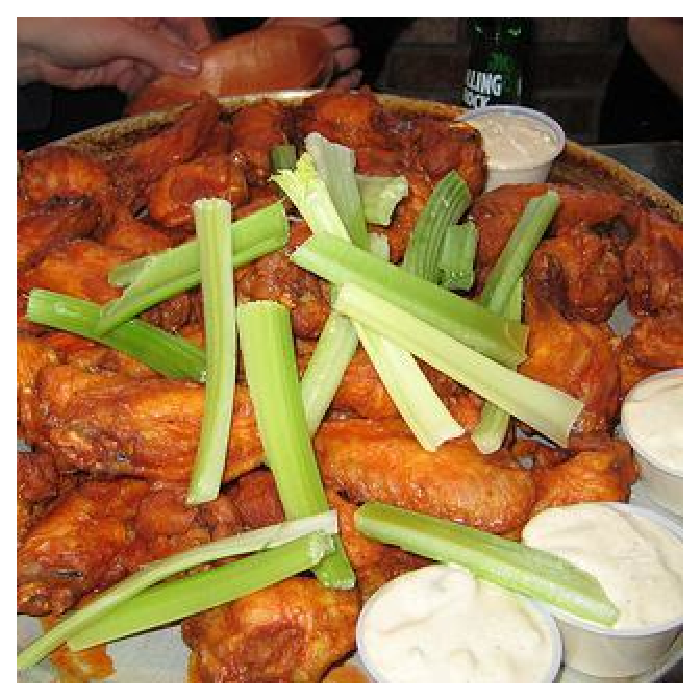
\epsfig{file=Figs4Paper/Buffalo_Wing/f192b38384.eps, height=1.25in, width=1.6in} 
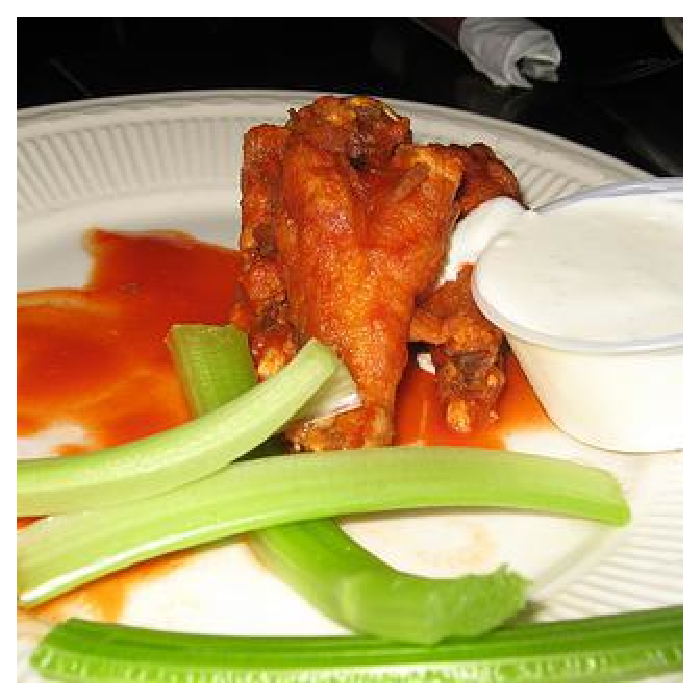
\epsfig{file=Figs4Paper/Buffalo_Wing/e1b0e74a83.eps, height=1.25in, width=1.6in}
\caption{Images of chicken wings dish with celery.}
\label{fig:chickenwingswithcelery}
\end{figure}
\section{Methods}

%Describe your learning algorithms, proposed algorithm(s), or theoretical proof(s). Make sure to include relevant mathematical notation. For example, say what the GAN objectives are or include your loss equation. It is okay to use formulas from the lecture notes. For each algorithm you use, give a brief description (2-3 sentences) of how it works. Again, we are looking for your understanding of how these deep learning algorithms work.
%Although the teaching staff probably know the algorithms, future readers may not (reports will be posted on the class website). Additionally, if you are using a niche or cutting-edge algorithm (e.g. WGAN, SURF features, or anything else not covered in the class), you may want to explain your algorithm using several paragraphs. Note: Theory/algorithms projects may have an appendix showing extended proofs (see appendix description below).


We plan to use Convolutional Neural Networks for an application based project.

%-------------------------------------------------------------------------
\section{Dataset and Features}

%Give details about your dataset: how many training/validation/test examples do you have? What is the class label distribution of the dataset? Is there any preprocessing you did? What about normalization or data augmentation? What is the resolution of your images? If using video, how is it discretized?  Include a citation to where you got your dataset from.
%
%Depending on available space, show some examples from your dataset. You should also talk about the features you used. If you extracted features using Fourier transforms, word2vec, histogram of oriented gradients (HOG), PCA, ICA, etc. make sure to talk about it. Try to include examples of your data in the report (e.g. include an image, etc.).

We provide some details about our dataset below.

\subsection{Dataset Details}
For the milestone, we are using a dataset of food dishes collected from ImageNet~\cite{imagenet}. We plan to collect more images using the Bing Image Search API~\cite{bingimagesearchapi} in the future.

\subsection{Class Label Distribution}
Currently our dataset has 15 classes. Table~\ref{table:classdistribution} shows the class label distribution of the dataset. We do note that currently the distribution of images across the classes is not uniform. We plan to address this in the following weeks.

\subsection{Preprocessing Steps}

We re-sized all of our images to 32*32*3, by cropping the image if it was larger than the standard size, or adding black padding if it was smaller. We found that ImageNet~\cite{imagenet} tends to contain spurious images; it has images which clearly do not belong to the class (e.g. images of human beings in the 'Fish And Chips' class). We removed some of these spurious images as part of data cleanup. Also, care must be taken for images which do not contain the RGB channels. Our training pipeline hit some issues when we encountered images without channel information. We subsequently used a fix to filter out such images. 

%\begin{figure}[!htb]
%\minipage{0.12\textwidth}
  %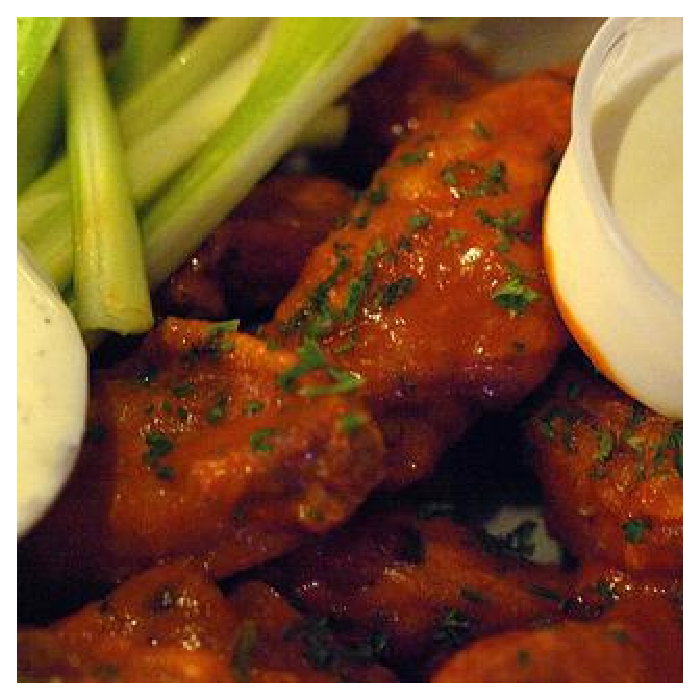
\includegraphics[width=\linewidth]{Figs4Paper/Buffalo_Wing/e1248c9ec5.eps}
%\endminipage\hfill
%\minipage{0.12\textwidth}
  %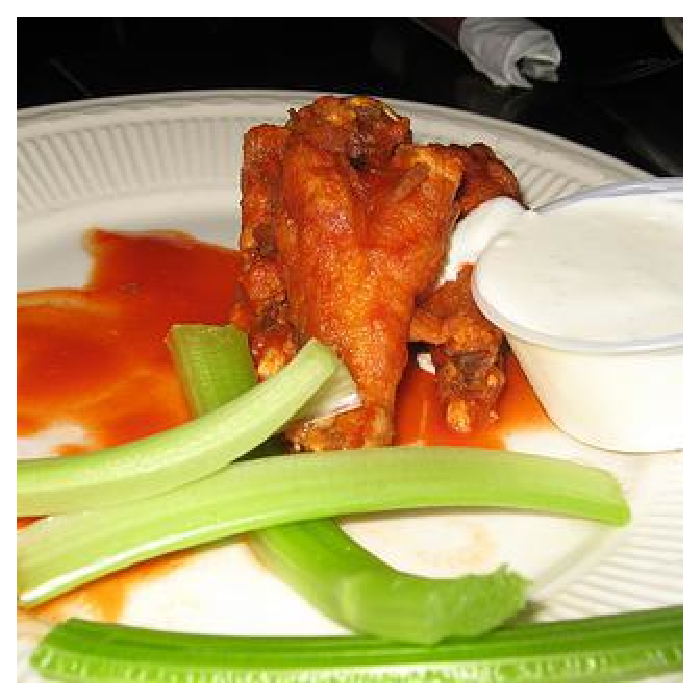
\includegraphics[width=\linewidth]{Figs4Paper/Buffalo_Wing/e1b0e74a83.eps}
%\endminipage\hfill
%\minipage{0.12\textwidth}%
  %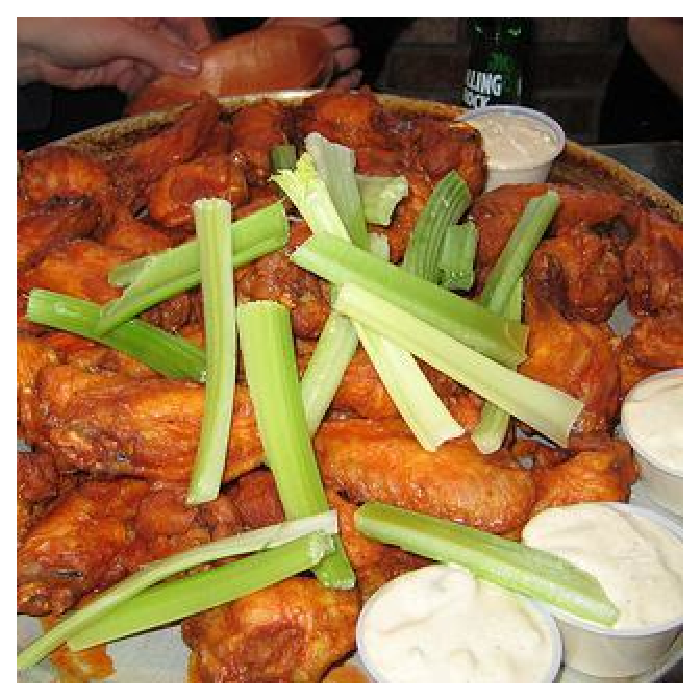
\includegraphics[width=\linewidth]{Figs4Paper/Buffalo_Wing/f192b38384.eps} 
%\endminipage
%\caption{Images of chicken wings dish with celery.}
%\label{fig:chickenwingswithcelery}
%\end{figure}

\begin{table}
\begin{center}
\begin{tabular}{|l|c|}
\hline
Food Name & Num of Images \\
\hline\hline
Clam Chowder&723\\
Jambalaya&588\\
Fish Stick&175\\
Cannelloni&230\\
Buffalo Wing&340\\
Lamb Curry&347\\
Fish And Chips&803\\
Pepperoni Pizza&773\\
Eggs Benedict&1124\\
Scotch Egg&388\\
Sashimi&818\\
Tempura&1008\\
Spaghetti&523\\
Beef Wellington&279\\
Lobster Thermidor&76\\
\hline
\end{tabular}
\end{center}
\caption{Class Label Distribution}
\label{table:classdistribution}
\end{table}

%-------------------------------------------------------------------------
\section{Experiments/Results/Discussion}

%You should also give details about what hyperparameters you chose (e.g. why did you use X learning rate for gradient descent or did you use Adam, what was your mini-batch size and why) and how you chose them. Did you do cross-validation, if so, how many folds? Before you list your results, make sure to list and explain what your primary metrics are: accuracy, precision, AUC, etc. Provide equations for the metrics if necessary.
%
%For results, you want to have a mixture of tables and plots. If you are solving a classification problem, you should include a confusion matrix or AUC/AUPRC curves. Include performance metrics such as precision, recall, and accuracy. For regression problems, state the average error. For reinforcement learning and control, have appropriate metrics as well.
%
%You should have both quantitative and qualitative results. To reiterate, you must have both quantitative and qualitative results! This includes unsupervised learning (talk with the TAs on how to quantify unsupervised methods). Include visualizations of results, heatmaps, examples of where your algorithm failed and a discussion of why certain algorithms failed or succeeded. In addition, explain whether you think you have overfit to your training set and what, if anything, you did to mitigate that. Make sure to discuss the figures/tables in your main text throughout this section. Your plots should include legends, axis labels, and have font sizes that are readable when printed.

In this section we discuss our experiments and results. While we ran multiple experiments, we are only providing details for the experiments which look best so far.

\subsection{Classifying food dishes using CNNs}

In the first problem, we want to classify food dishes using Convolutional Neural Networks. We formulate this problem as a standard classification task with one class per image. We use accuracy as our evaluation metric.

We split our dataset randomly into 3 disjoint sets: Train(70\% approx.), Validate(20\% approx.) and Test(10\% approx.). Table~\ref{table:classificationresults} provides a count of the number of images in each set.

\subsubsection{Experiment}
\label{subsubsec:pb1experiment}

We are currently using a very simple model which has the following architecture:

\begin{itemize}[noitemsep]
\item 7x7 Convolutional Layer with 32 filters and stride of 2
\item ReLU Activation Layer
\item Affine layer with 15 outputs
\end{itemize}

Also, we are using the Hinge loss function in conjunction with the Adam optimizer to minimize loss.

\subsubsection{Results}
\label{subsubsec:pb1results}

Figure~\ref{fig:lossepoch1} shows the reduction in the loss over multiple iterations in the first epoch. We see the loss reduces very sharply in the beginning, and then flattens out gradually.  Currently we are running only a single epoch to train our model.  

\begin{figure}[h!]
%\color{red}
\centering
  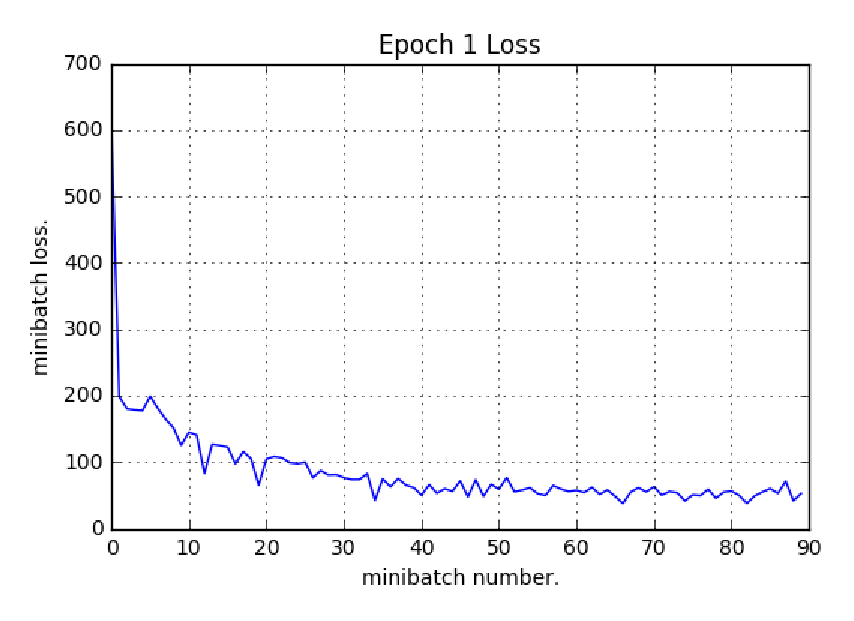
\epsfig{file=Figs4Paper/Plots/lossEpoch1.eps, height=1.5in, width=2.5in}
  \caption{Reduction in loss over several mini-batches in the first epoch}
  \label{fig:lossepoch1}
%  }
\end{figure}


Table~\ref{table:classificationresults} shows the accuracy metric for train, validation and test sets.

\begin{table}
\begin{center}
\begin{tabular}{|l|c|c|}
\hline
Dataset & Num of Images & Accuracy \\
\hline\hline
Train & 5756 & 0.18 \\
Validate & 1619 & 0.2 \\
Test & 819 & 0.0842 \\
\hline
\end{tabular}
\end{center}
\caption{Dataset Details}
\label{table:classificationresults}
\end{table}

\subsubsection{Discussion}
\label{subsubsec:pb1discussion}

We observe that train (and validate) accuracy is much higher than the test accuracy. This suggests that we are probably overfitting the training set. We plan to investigate this in depth going forward, including the use of (a) dropout (b)  L2 weight regularization  (c) increasing size of the dataset etc. Any feedback on how to improve the test accuracy is highly welcome.

\subsection{Detecting individual food items in an image.}

For this problem we are planning to use some standard CNN based detection methods such as SSD~\cite{liu2016ssd}, Fast-RCNN~\cite{ren2015faster} and YOLO~\cite{redmon2016you}. These approaches typically detect bounding boxes of interest in an image, and we want to leverage these techniques to detect the individual food items in an image. For this milestone we were not able to make much progress on this problem. We plan to work on this in the coming weeks. 



\section{Conclusion/Future Work}

For the first problem of classifying dishes, we have made some progress in our workflow : data collection, pre-processing and building simple models. As future work, we need to investigate why we are seeing low accuracies in the test set, and explore techniques to improve the same.

For the second problem of detecting individual food items from images, we plan to start looking into CNN based detection methods.

%------------------------------------------------------------------------
{\small
\bibliographystyle{ieee}
\bibliography{egbib}
}

\end{document}
